%\documentclass[letterpaper,draft]{beamer}
%\documentclass[letterpaper,handout]{beamer}
\documentclass[letterpaper, mathserif]{beamer}

%---multiple pages on one sheet, ADD for handout--
%\usepackage{pgfpages}
%\pgfpagesuselayout{4 on 1}[letterpaper, landscape, border shrink=1mm]
%-------------------------------------------------
\usepackage{amsmath,amsfonts}
\usepackage{graphicx}
%\usepackage{booktabs}
%\usepackage{mdwlist}
%\usepackage{pgf,tikz}
%\usetheme{Copenhagen}
%\usetheme{warsaw}
\setbeamertemplate{navigation symbols}{}
\usepackage[english]{babel}
\def\ul{\underline}
% or whatever

\usepackage[latin1]{inputenc}
\subject{Talks}

\def\P{\mathbb{P}}
\def\p{\mathrm P}
\def\E{\mathbb E}
\def\Sum{\sum\nolimits}
\def\X{\mathfrak{X}}
\def\typo#1{\alert{#1}}
%-------------Answers------------
\def\Hide#1#2{\ul{~~~\onslide<#1>{\alert{#2}}~~~}}
\def\hide#1#2{\ul{~~\onslide<#1>{\alert{#2}}~~}}
\def\hid#1#2{\onslide<#1>{\alert{#2}}}
%------Centered Page Number------
\defbeamertemplate{footline}{centered page number}
{%
  \hspace*{\fill}%
  %\usebeamercolor[fg]{page number in head/foot}%
  %\usebeamerfont{page number in head/foot}%
  \small Lecture \chapnum\ - \insertframenumber%
  \hspace*{\fill}\vskip2pt%
}

%\usepackage{tikz}
%\usebackgroundtemplate{%
%\tikz\node[opacity=0.3] {\includegraphics[height=\paperheight,widht=\paperwidth]{ctanlion}};}

%\usebackgroundtemplate{%
%  %\rule{0pt}{\paperheight}%
%  \parbox[c][\paperheight][c]{\paperwidth}{\centering\includegraphics[width=.65\paperwidth]{UClogo.pdf}}
%  %\hspace*{\paperwidth}
%}

\title{STAT253/317 Winter 2014 Lecture \chapnum}
\date{January 13, 2014}
\author{Yibi Huang}
\def\chapnum{3}
%--------------------------------
\setbeamertemplate{footline}[centered page number]
\begin{document}
% ----------------------------------------------------------------------
%\begin{frame}\maketitle\bigskip
%\begin{center}
%4.3 Classification of States
%\end{center}
%\end{frame}
% ----------------------------------------------------------------------
\begin{frame}{STAT253/317 Lecture 3: 4.3 Classification of States}
\medskip

Introduce state diagram. \\

\noindent\textbf{Definition}. Consider a Markov chain $\{X_n, n\ge 0\}$ with state space $\X$.
For two states $i,j\in \X$, we say state $j$ is \structure{\bf accessible} from state $i$ if $P^{(n)}_{ij}>0$ for some $n$, and we denote it as $$i\to j.$$

Note that \structure{\bf accessibility is transitive}: for $i,j,k\in\X$,\\
\centerline{if $i\to j$ and $j\to k$, then $i\to k$.}
{\em Proof.}
\begin{align*}
i\to j\quad &\Rightarrow\quad P^{(m)}_{ij}>0\text{ for some }m\\
j\to k\quad &\Rightarrow\quad P^{(n)}_{jk}>0\text{ for some }n
\end{align*}
By Chapman-Kolmogorov Equation:
$$P_{ik}^{(m+n)}=\Sum_{l\in\X}P_{il}^{(m)}P_{lk}^{(n)}\ge P_{ij}^{(m)}P_{jk}^{(n)}>0,$$
which shows $i\to k$.
\end{frame}
% ----------------------------------------------------------------------
\begin{frame}{Communicability}\medskip
\noindent\textbf{Definition}. Consider a Markov chain $\{X_n, n\ge 0\}$ chain with state space $\X$.
Two states $i,j\in \X$ are said to \structure{\bf communicate} if $i\to j$, and $j\to i$.
We denote it as $$i\longleftrightarrow j.$$\bigskip


\noindent\textbf{Fact}.
Communicability is also \structure{transitive}, meaning that
\[
\text{if }i\longleftrightarrow j\text{ and }j\longleftrightarrow k\text{, then }i\longleftrightarrow k.
\]
The proof is straight forward from the transitivity of accessibility.
\end{frame}
% ----------------------------------------------------------------------
\begin{frame}{Communicative Class}\medskip

\noindent\textbf{Definition}.
Two states that communicate with each other are in the same \structure{\bf class}.
A state that communicates with no other states itself is a class.\medskip

\noindent\textbf{Fact}. Two classes are either identical or disjoint.\smallskip

{\em Proof.}
If two classes $A$ and $B$ have one state $i$ in common, then
all states in $A$ communicate with $i$ and all states in $B$ do too.
Consequently, all states with $A$ can communicate with states in $B$ (through state $i$).
Class $A$ and Class $B$ must be identical.

\begin{center}
\only<1>{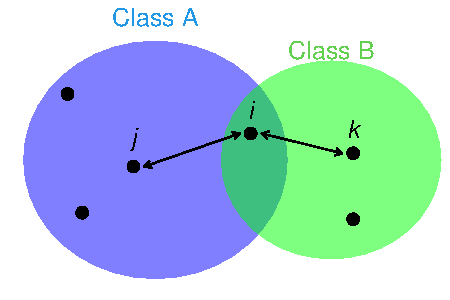
\includegraphics[width=0.6\textwidth]{communicate_class.pdf}}%
\only<2>{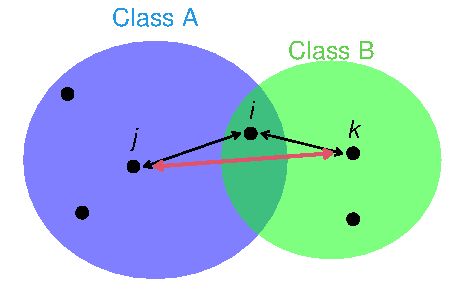
\includegraphics[width=0.6\textwidth]{communicate_class2.pdf}}%
\only<3->{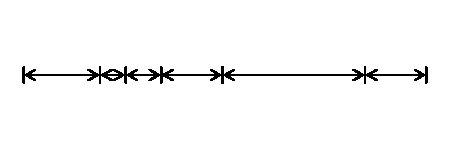
\includegraphics[width=0.6\textwidth]{communicate_class3.pdf}}
\end{center}
\end{frame}
% ----------------------------------------------------------------------
\begin{frame}\text{}\hspace{-5pt}
{\bf Example 1}. Specify the classes of the following Markov chains.
\[
\P_1=
\bordermatrix{%
  &  1  &  2  &  3  &  4 \cr
1 & 0.5 & 0.5 &  0  &  0 \cr
2 & 0.3 & 0.6 & 0.1 &  0 \cr
3 &  0  &  0  & 0.2 & 0.8\cr
4 &  0  &  0  & 0.9 & 0.1
}
\quad\P_2=
\bordermatrix{%
  &  1  &  2  &  3  &  4 \cr
1 & 1/2 & 1/2 &  0  &  0 \cr
2 & 1/2 & 1/2 &  0  &  0 \cr
3 & 1/4 & 1/4 & 1/4 & 1/4\cr
4 &  0  &  0  &  0  &  1
}
\]

\hid{2-}{For $\P_1$, $1 \leftrightarrow 2 \to 3 \leftrightarrow 4$. Classes: \{1,2\}, \{3,4\}.}\medskip

\hid{3-}{For $\P_2$,
$\displaystyle
\begin{array}{ccc}
1 &\longleftrightarrow& 2\\[-2pt]
  &\nwarrow&\uparrow\\
4 &\leftarrow& 3\\[-3pt]
{\Large\circlearrowleft} & & {\Large\circlearrowleft}
\end{array}.
$
Classes: \{1,2\}, \{3\}, \{4\}.}\bigskip

{\bf Example 2}. How many classes does the Ehrenfest diffusion model with $K$ balls have?\pause

\hid{4-}{All states communicate. Only one class.}
\end{frame}
% ----------------------------------------------------------------------
%\begin{frame}{Closed Classes}
%
%\noindent\textbf{Definition}. A class $C$ is said to be \structure{closed} if
%\[P_{ij} = 0\quad \text{for all $i$ in $C$ and $j$ not in $C$}.
%\]
%Once the process gets into a closed class. It will never leave the class since
%the outgoing probabilities from the class are all 0.\medskip
%
%{\bf Examples}.
%\begin{itemize}
%\item For $\P_1$ in the previous slide, the class \{1,2\} is not closed
%because it has a non-zero outgoing probability $P_{23}=0.1>0$. The class $\{3,4\}$ is closed.
%\item For $\P_2$ in the previous slide, the classes $\{1,2\}$ and $\{4\}$ are closed, and $\{3\}$ is not closed.
%\end{itemize}
%\end{frame}
%% ----------------------------------------------------------------------
%\begin{frame}{A Markov Chain Restricted to a Closed Class is Also a Markov Chain}\smallskip
%
%{\bf Example}.
%\[
%\P_1=
%\bordermatrix{%
%  &  1  &  2  &  3  &  4 \cr
%1 & 0.5 & 0.5 &  0  &  0 \cr
%2 & 0.3 & 0.6 & 0.1 &  0 \cr
%3 &  0  &  0  & 0.2 & 0.8\cr
%4 &  0  &  0  & 0.9 & 0.1
%}
%\]
%\begin{itemize}
%\item For $\P_1$ above, the Markov chain restricted to the class \{3,4\} is also a Markov chain, with transition matrix \[
%\bordermatrix{%
%  &  3  &  4 \cr
%3 & 0.2 & 0.8\cr
%4 & 0.9 & 0.1
%}
%    \]
%\item The Markov chain for $\P_1$ can not be restricted to \{1,2\} as it may transit out of the state space from 2 to 3.
%\end{itemize}
%\end{frame}
% ----------------------------------------------------------------------
\begin{frame}{Irreducibility}
A Markov chain is said to be \structure{\bf irreducible} if it has only 1 class.
\end{frame}
% ----------------------------------------------------------------------
\begin{frame}{Recurrence \& Transience}
Consider a Markov chain $\{X_n, n\ge 0\}$ chain with state space $\X$.
For $i\in\X$, define $$f^{(n)}_{ii}=\p(X_n=i, X_v \neq i \text{ for }v = 1,2,\ldots, n-1 \mid X_0=i)$$
If $\sum_{n \geq 1} f^{(n)}_{ii}=1$, we say state $i$ is \structure{\bf recurrent}\\
If $\sum_{n \geq 1} f^{(n)}_{ii} < 1$, we say state $i$ is \structure{\bf transient}
\begin{itemize}
\item It's generally difficult to compute $\sum_{n \geq 1} f^{(n)}_{ii}$ directly.\\
We need other tools to determine whether a state is recurrent or transient.
\end{itemize}
\end{frame}


\begin{frame}{An equivalent characterization}
Proposition 4.1: State $i$ is
\begin{align*}
\begin{cases}
\text{recurrent if}& \Sum_{n=1}^{\infty}P^{(n)}_{ii}=\infty\\
\text{transient if}& \Sum_{n=1}^{\infty}P^{(n)}_{ii}<\infty
\end{cases}
\end{align*}

{\bf Proof: }
Suppose that $X_0 = i$, and consider the random variable 
$N(i) = \sum_{n = 1}^{\infty} 1\{ X_n = i\}$

We will use two way to calculate the expectation of $N(i)$. 
First, by definition we have
\begin{align*}
\mathbb{E} [ N(i) ] &= \mathbb{E} [ \sum_{n = 1}^{\infty} 1\{ X_n = i\} ] 
=  \sum_{n = 1}^{\infty} \mathbb{E} [ 1\{ X_n = i\} ] \\
&= \sum_{n = 1}^{\infty} \p \{ X_n = i\} ] =  \Sum_{n=1}^{\infty}P^{(n)}_{ii}
\end{align*}
In addition, we have 
\begin{align*}
\mathbb{E} [ N(i) ] &= \sum_{k = 0}^{\infty} \p ( N(i) \geq k ) =
 \sum_{k = 0}^{\infty} ( \sum_{n \geq 1} f^{(n)}_{ii} )^k
\end{align*}
\end{frame}

%
%\begin{frame}
%
%Implication of Proposition 4.1:
%
%\begin{center}States in a \underline{finite-state} Markov chain CANNOT be all transient.\end{center}
%
%{\em Reason.} Observe that $\Sum_{i\in X}I_{ni}=1$ for all $n$ since $X_n$ must be in one of the states.
%Thus $$\Sum_{n=1}^{\infty}\Sum_{i\in X}I_{ni}=\Sum_{n=1}^{\infty}1=\infty.$$
%Since $\X$ is finite, there exists at least one state $i$ such that $$\Sum_{n=1}^{\infty}I_{ni}=\infty.$$
%Such states are recurrent. Otherwise $\Sum_{n=1}^{\infty}\Sum_{i\in X}I_{ni}$ will be $<\infty.$
%\end{frame}
% ----------------------------------------------------------------------
\begin{frame}{Corollary 4.2}
If $i\longleftrightarrow j$, and $i$ is recurrent, then $j$ is also recurrent.\medskip

{\em Proof}.
\begin{align*}
i\to j\quad &\Rightarrow\quad P^{(k)}_{ij}>0\text{ for some }k\\
j\to i\quad &\Rightarrow\quad P^{(l)}_{ji}>0\text{ for some }l
\end{align*}
By Chapman-Kolmogorov Equation:
$$P_{jj}^{(l+n+k)}\ge P_{ji}^{(l)}P_{ii}^{(n)}P_{ij}^{(k)}, \text{ for all }k=0,1,2,\ldots$$
Thus
$$
\Sum_{n=1}^{\infty}P^{(n)}_{jj}
\ge \Sum_{n=1}^{\infty}P^{(l+n+k)}_{jj}
\ge \underbrace{P_{ji}^{(l)}}_{>0}\underbrace{\Sum_{n=1}^{\infty}P_{ii}^{(n)}}_{=\infty}\underbrace{P_{ij}^{(k)}}_{>0}
=\infty
$$
\hrule\medskip
Corollary 4.2 implies that all states of a finite irreducible Markov chain are recurrent.
\end{frame}

\begin{frame}{Finite irreducible MC}

\textbf{Theorem} All states of a finite irreducible Markov chain are recurrent. 

%\textbf{Proof:} First based on the previous corollary, we know either all the states 
%are transient, or all the states are recurrent. Suppose that all the states are 
%transient. Then one has for 
\end{frame}


% ----------------------------------------------------------------------
%\begin{frame}{States in a Non-Closed Class Are Always Transient}
%For a class $A$ that is NOT closed,
%there must exists some state $k$ not in $A$ such that
%$$P_{i_0,k}>0,\quad\text{for some state $i_0$ in class }A$$
%but
%$$
%P^{(n)}_{ki}=0\quad\text{for all state $i$ in class $A$ and for all $n$}.
%$$
%Otherwise, state $i$ would be accessible from state $k$ ($k\longrightarrow i$).
%As $i$ and $i_0$ are in the same class, we know $i\longleftrightarrow i_0$.
%Combining all the above, we have
%$$
%k\longrightarrow i \longleftrightarrow i_0\stackrel{P_{i_0,k}>0}{\longrightarrow} k.
%$$
%and hence $k$ would communicate with $i_0$, contradicting to the assumption that $k$ is not in $A$.
%
%\pause
%
%Starting from a state $j$ in a non-closed class $A$,
%there is a positive probability that the Markov chain will move to state $k$
%and never comes back to the class. Hence state $j$ must be transient.
%\bigskip\pause
%\hrule\medskip
%
%Are states in an closed class always recurrent?
%\end{frame}
%% ----------------------------------------------------------------------
%\begin{frame}
%\begin{itemize}
%\item[Fact 1] If state $i$ is recurrent, then starting from state $i$, the process will revisit state $i$ infinitely often.\vspace{0.5in}
%\item[Fact 2] If state $i$ is transient, then starting from state $i$, the number of times the process revisits state $i$ is finite, with expected value $1/(1-f_i).$\\
%Reason: Let $N_i$ be the number of times the process revisits state $i$ after starting from $i$.
%Observe that
%\begin{align*}
%\p(N_i=k)
%&=\p(\text{returns to $i$ after 1st departure})\\
%&\quad\times\cdots\times\p(\text{returns to $i$ after $k$th departure})\\
%&\quad\times\p(\text{never returns to $i$ after k+1st departure})\\
%&=f_i^k(1-f_i),\quad k=0,1,2,\ldots
%\end{align*}
%i.e., $N_i$ has a geometric distribution with mean $1/(1-f_i).$
%\end{itemize}
%\end{frame}
% ----------------------------------------------------------------------
%
%\begin{frame}
%Claim: $$\E(\text{\# of visit to state }i|X_0=i)=\Sum_{n=1}^{\infty}P^{(n)}_{ii}$$
%
%{\em Proof.} Define
%$$I_{ni}=\begin{cases}1 &\text{if }X_n=i\\0&\text{if }X_n\neq i\end{cases},\quad n\ge 0,\;i\in\X.$$
%Observe that $\Sum_{n=1}^{\infty}I_{ni}$ is the number of visits to state $i$.
%\begin{align*}
%\E\left[\Sum_{n=1}^{\infty}I_{ni}\Big|X_0=i\right]
%  &=\Sum_{n=1}^{\infty}\E[I_{ni}|X_0=i]\\
%  &=\Sum_{n=1}^{\infty}\p(X_n=i|X_0=i)\\
%  &=\Sum_{n=1}^{\infty}P^{(n)}_{ii}
%\end{align*}
%\begin{block}{Conclusion from Fact 1, Fact 2 and the Claim Above:}
%
%\vspace{-20pt}
%\begin{align*}
%\text{State $i$ is recurrent }&\iff \E(\text{\# of visit to state }i|X_0=i)=\infty.\\
%&\iff \Sum_{n=1}^{\infty}P^{(n)}_{ii}=\infty
%\end{align*}
%\end{block}
%\end{frame}
% ----------------------------------------------------------------------
% ----------------------------------------------------------------------
\begin{frame}{Example: One-Dimensional Random Walk}
$$
X_{n+1}=
\begin{cases}
X_n+1 &\text{with prob. } p\\
X_n-1 &\text{with prob. } 1-p\\
\end{cases}
$$
\begin{itemize}
\item State space $\{\cdots, -3, -2, -1, 0, 1, 2, 3,\cdots\}$
\item All states communicate
$$
\cdots \longleftrightarrow-2\longleftrightarrow -1 \longleftrightarrow 0\longleftrightarrow 1\longleftrightarrow 2\longleftrightarrow\cdots
$$
\begin{align*}
\text{Only one class} &\Rightarrow\text{ Irreducible}\\
&\Rightarrow\text{ States are all transient or all recurrent.}
\end{align*}

It suffices to check whether 0 is recurrent or transient, i.e., whether
$$
\sum_{n=1}^{\infty}P^{(n)}_{00}=\infty \text{ or } <\infty
$$
\end{itemize}
\end{frame}
% ----------------------------------------------------------------------
\begin{frame}{Example: One-Dimensional Random Walk (Cont'd)}
\begin{align*}
P^{(2n+1)}_{00}&=0 \quad\text{(Why?)}\\
P^{(2n)}_{00}&={2n\choose n}p^n(1-p)^n \\
&=\frac{(2n)!}{n!\,n!}p^n(1-p)^n \quad\fbox{\text{\small Stirling's Formula:} $n!\approx n^{n+0.5}e^{-n}\sqrt{2\pi}$}\\
&\approx \frac{(2n)^{2n+0.5}e^{-2n}\sqrt{2\pi}}{(n^{n+0.5}e^{-n}\sqrt{2\pi})^2}p^n(1\!-\!p)^n\\
&=\frac{1}{\sqrt{\pi n}}[4p(1-p)]^n
\end{align*}
Thus
$$
\sum_{n=1}^{\infty}P^{2n}_{ii}\approx\sum_{n=1}^{\infty}\frac{1}{\sqrt{\pi n}}[4p(1-p)]^n
\begin{cases}
< \infty & \text{if }p\neq 1/2\\
= \infty & \text{if }p= 1/2
\end{cases}
$$
Conclusion: One-dimensional random walk is recurrent if $p=1/2$, and transient otherwise.
\end{frame}
% ----------------------------------------------------------------------
\begin{frame}{Example: Two-Dimensional Symmetric Random Walk}
Irreducible. Just check if 0 is recurrent.

\begin{align*}
P^{(2n)}_{00}
&=\sum_{i=0}^{n}\frac{(2n)!}{i!i!(n-i)!(n-i)!}\left(\frac{1}{4}\right)^{2n}\\
&={2n\choose n}\underbrace{\sum_{i=0}^{n}{n\choose i}{n\choose n-i}}_{={2n\choose n}}\left(\frac{1}{4}\right)^{2n}\\
&={2n\choose n}^2\left(\frac{1}{4}\right)^{2n}\approx\frac{1}{\pi n}\quad\text{by Stirling's Formula}\\
\end{align*}
Thus $\sum_{n=1}^{\infty}P^{(2n)}_{00}=\infty$.\medskip

Two-dimensional symmetric random walk is {\bf recurrent}.
\end{frame}
% ----------------------------------------------------------------------
\begin{frame}{Example: $d$-Dimensional Symmetric Random Walk}
In general, for a $d$-dimensional symmetric random walk, it can be shown that
$$
P^{(2n)}_{00}\approx(1/2)^{d-1}\left(\frac{d}{n\pi}\right)^{d/2}
$$
Thus
$$\sum_{n=1}^{\infty}P^{(2n)}_{00}\begin{cases}
= \infty & \text{for }d= 1\text{ or }2\\
< \infty & \text{for }d\ge 3
\end{cases}.
$$
\bigskip

\begin{center}
``{\em A drunken man will find his way home.\\
\quad A drunken bird might be lost forever.}''
\end{center}
\end{frame}
% ----------------------------------------------------------------------
\end{document} 